%% -------------------------------------------------------------
%% Introduction.tex
%% -------------------------------------------------------------
\chapter{Introduktion} \label{Chapter:Introduction}

Fossila bränslen står idag för 82 \% av världens totala energibehov \citep{Fossila}. Eftersom förbränningen av fossila bränslen är huvudanledningen till växthuseffekten behövs alternativa energikällor. Därför står vindkraft idag för en allt växande global trend av installerad kapacitet vilket syns i \fref{installerad vindkraft}.

\begin{figure}[!htb]
  \centering
  \includegraphics[width=0.9\textwidth]{installeradvind}
  \caption{Totalt installerad global vindkraftseffekt. Reproducerat från \citet{ackvind}.}
  \label{installerad vindkraft}
\end{figure}

Förnyelsebara energikällor såsom vindkraftverk är ideala eftersom de inte medför betydande utsläpp av växthusgaser. Vindkraftverk är samtidigt idag ett av de absolut mest kostnadseffektiva sättet att producera energi. Koldixoxidutsläppen som produktionen och uppförandet av ett vindkraftverk ger upphov till är uppvägda efter tre till sex månader efter att vindkraftverket tagits i drift. Efter detta återstår c:a 20 års fossilfri kraftproduktion vilket är en vanlig livstid för ett vindkraftverk \citep{GWEC}. 

\begin{comment}
\rework{Dock är vindkraft, likt alla andra kraftkällor - förknippat med sina negativa sidor. Energi kan endast produceras när vinden blåser vilket leder till att energi då måste komma från andra energikällor. När istället det motsatta råder, ett överskott på vindenergi - måste energin lagras eller transporteras vidare till där den behövs. Andra nackdelar är störande ljud som de ger upphov till, skuggor som sveper, elektromagnetisk strålning och fåglar och fladdermöss som dör i kollisioner med rotorbladen. Dessa nackdelars betydelse har med åren minskat eftersom lösningar finns på många av dem, och trots nackdelarna - överväger de positiva effekterna. [Ska nog bort]}
\end{comment}

\begin{comment}
Installerad effekt växer

Tyskland fasar ut efter Fukushima. Till 2020 ingen kärnkraft.

Vindkraftens nackdelar. Endast när det blåser.Oljud. Viosuellt. Skuggor som flimmrar. Djur som dör. Går att göra något åt och problemen minskar succesivt. Positivt överväger det negativa.
\end{comment}


\section{Syfte}
För att gynna möjligheterna till en hållbar framtid syftar denna studie bidra till effektiviseringar av ett vindkraftverks energiproduktion.
%men även främja öppenhet och vindlighet av information.

\section{Mål}
Det generella målet är att utifrån ett histogram med vindhastigheter för en plats kunna presentera det rotorblad som ger största genomsnittliga effekt för ett vindkraftverk. Detta kommer ske genom ett par delmål:

\begin{itemize}

  \item Skapa en modell som förutsäger ett vindkraftverks genomsnittliga effekt.

  \item Hitta och presentera ett referensfall som kan användas för att utvärdera den skapade modellens giltighet.
  
  \item Ett optimeringsproblem ska formuleras och implementeras som kommunicerar med modellen för att hitta rotorblad med högre genomsnittlig effekt.
  
  \item Ta fram ett alternativt rotorblad genererat ur optimeringen och jämföra dess prestanda mot referensfallet.
 
\end{itemize}




\section{Litteraturstudie}

\subsection{Vindturbiner}
Vindkraftverk är en maskin som konverterar vindens inneliggande rörelseenergi till elektrisk energi. Detta görs genom att inkommande luft skapar en lyftkraft på rotorbladets vingprofil som driver ett vridmoment. Vridmomentet utnyttjas sedan i en generator för att producera el. I \fref{liftdrag} syns ett tvärsnitt av ett vindkraftverks rotorblad med lyft- ($L$) och motstånds- ($D$) och normalkraft ($N$) utmarkerat. 

    \begin{figure}[!htb]
      \centering
      \includegraphics[width=0.9\textwidth]{liftdrag.pdf}
      \caption{Vingprofil med krafter utmarkerat.  Fritt reproducerat från \citet{hansen}.}
      \label{liftdrag}
    \end{figure}

\begin{figure}[!htb]
  \centering
  \subfigure[Horizontellt axlad vindturbin (\textsc{hawt})]{
    \includegraphics[height=7cm]{hawt.pdf}
    \label{hawt}
  }
  \subfigure[Vertikalt axlad vindturbin (\textsc{vawt})]{
    \includegraphics[height=7cm]{vawt.pdf}
    \label{vawt}
  }
  \caption{De två vanligaste typerna av vindturbiner. Fritt reproducerat från \citet{wehb}.}
  \label{hawtvawt}
\end{figure}


I \fref{hawt} syns den horisontellt axlade vindturbinen (ofta kallat \textsc{hawt}) vilken är den vanligast förekommande. En alternativ variant på vindkraftverk är den vertikalt axlade vindturbinen (\textsc{vawt}) som syns i \fref{vawt}. Dessa har fördelarna att de producerar effekt oavsett vindriktning samt att de är lättare att utföra service på då viktiga delar nås från fundamentet. Dessa utvecklades i kommersiell skala fram till 80-talet men får idag mindre uppmärksamhet på grund av dess nackdelar:

    \begin{itemize}
    
      \item Närmast marken är vindhastigheten lägre (vidhäftningsvilkoret) vilket gör att turbinens nedre del är mindre effektiv än den övre.
    
      \item Turbinen har svårt att självstarta och behöver därför en motor för att komma upp i en hastighet där de producerar effekt.
      
      \item Vridmomentet fluktuerar mycket mellan rotationerna.
      
      \item De kräver en mekanisk broms vid höga vindhastigheter för att inte komma upp i rotationshastigheter där konstruktionen går sönder.
     
    \end{itemize}


\textsc{hawt} är den idag mest förekommande varianten och den enda som behandlas i denna uppsats. I stora drag består en \textsc{hawt} av en motorgondol monterat på ett högt torn. I motorgondolen finns en generator samt även ofta ett växelhus, även om ett ökande antal vindturbiner idag är utan växelhus. För att vända turbinen mot den inkommande vinden finns oftast en motor som möjliggör gir ($\gamma$) (se \fref{gir}). 

\begin{figure}[!htb]
  \centering
  \includegraphics[width=12cm]{gir.eps}
  \caption{Gir ($\gamma$), korda ($c$) och pitch ($\theta_p$)  utmarkerat på en vindturbin.}
  \label{gir}
\end{figure}

En rotor som sitter framför motorgondolen uppströms vindens riktning samt tre rotorblad är idag den vanligast förekommande typen av vindturbin i kommersiell drift. Vanligast är även att rotationshastigheten ($\Omega$) är variabel.

För att kunna kontrollera vindkraftverket vid höga rotationshastigheter sitter ofta även motorer som kontrollerar rotorbladens så kallade pitch ($\theta_p$). När vindhastigheten blir för hög kan rotorbladen ställas så att lyftkraften minskar och på så sätt hålla generatorn från att skadas. Korda ($c$) beskriver rotorbladets vingprofils längd i ett tvärsnitt och varierar ofta med radien. Dessa koncept illustreras i \fref{gir}. En ytterligare vridning längs radien kallas \emph{twist} ($\beta$) och definieras som avvikelse från kordans plan i rotorbladets topp.

Idag existerar vindturbiner med maximal effekt från några enstaka kW till flera MW och rotordiametern är därefter. Ett vindkraftverk i MW-klass är inte sällan över 100 m i diameter \citep{kap10}.

\subsection{Vindens inneliggande energi}
Vindens inneliggande kinetiska energi som passerar den cirkulära area rotorn sveper i \fref{hawt} kan visas ge effekten

\begin{equation}\label{pvind} P_{vind} = \frac{1}{2}\rho A V_{\infty}^{3}  =  \frac{1}{2}\rho V_{\infty}^{3}\pi R^2 \end{equation}

Där $A$ är den cirkulära arean $\pi R^2$ där $R$ är radien och $V_\infty$ vindhastigheten uppströms rotorn. Ekvationen visar alltså att energin som kan tas ut ur vinden beror på vindhastigheten i kubik vilket är viktigt att komma ihåg. Den visar även att effektuttaget är beroende på radien i kvadrat, vilket förklarar dagens trend med ökande storlek på vindkraftverken.

I praktiken är effekten som ett vindkraftverk genererar aldrig så hög som ekvation \ref{pvind} antyder. Det hade inneburit att vinden tappat all sin hastighet genom rotorn och blockerat ytterligare vind. Detta leder oss till den dimensionslösa storheten $C_P$ som är vanlig i dessa sammanhang definierad

\begin{equation}\label{cp} C_P =  \frac{P}{P_{vind}} = \frac{P}{\frac{1}{2}\rho V_{\infty}^{3}\pi R^2} \end{equation}

Detta är alltså andelen producerad effekt mot det som annars hade passerat den cirkulära arean.

Nästa vanliga storhet att vara bekant med är löptalet $\lambda$ (på engelska tip speed ratio) vilket $C_P$ visar sig vara starkt beroende av. Denna definieras

\begin{equation}\label{tsr} \lambda = \Omega R / V_\infty = V_{topp}/V_\infty \end{equation}

Vilket relaterar rotorns toppars hastighet $\Omega R$ mot den inkommande friströmshastigheten $V_\infty$. $\lambda$ brukar vara mellan 7 och 10 när vindkraftverk producerar maximalt $C_P$. 

Den tredje dimensionslösa enheten är Reynolds tal som i vindkraftssammanhang definieras

\begin{equation}\label{reynolds} Re = V_{total} c/\nu \end{equation}

$V_{total}$ kommer att definieras tydligare i \ref{BEMlitt} men är den totala hastigheten en vingprofil ser när både inkommande hastighet $V_\infty$ och $\lambda$ gör sig gällande. $c$ betecknar kordan och $\nu$ luftens kinematiska viskositet. 

\subsection{Effekt-kurvan för ett vindkraftverk}

I \fref{vestas} visas en Vestas V80 2 MW vindkraftverks effektkurva. Detta är ett vindkraftverk med 80 meter i diameter och med en typisk effektkurva. Inkoppling sker när lägsta vindhastighet som kan producera effekt uppnås $U_{in}$ (på engelska \emph{cut-in wind speed}), vilket i detta fallet är 3 m/s.  

\begin{figure}[!htb]
  \centering
  \includegraphics[width=11cm]{powerwindspeed.eps}
  \caption{Effektkurva för Vestas V80 2 MW 80 m diameter. Fritt reproducerat från \citet{smallwindturbines}.}
  \label{vestas}
\end{figure}

Effekten planar i \fref{vestas} ut mot det som kallas märkeffekt (på engelska \emph{rated power}) vilket är det maximala effekt generatorn kan producera. När denna effekt närmas vrids rotorbladen via deras pitch ($\theta_p$) för att minska lyftkraften och på så vis kunna hålla sig under märkeffekten. Alternativt används en mekanisk broms. Detta görs för att generatorn inte ska skadas.

Vid en maximal vindhastighet $U_{ut}$ kommer även vindkraftverket att stänga av helt och hållet (eng: \emph{cut-out speed}) eftersom risken för skador från den höga rotationshastigheten och dess medförda centrifugalkrafter då är för stora. Detta kan göras genom att bladen ställs så att endast motståndskraft uppstår vilket får rotationen att upphöra. 

\pagebreak
\subsection{$C_P$-kurvan}

En kurva visandes $C_P$ mot $\lambda$ visas i \fref{cpTSR}. Som tidigare nämnt finns alltid ett löptal $\lambda$ där ett maximalt $C_P$ uppnås. Därför körs moderna vindkraftverk med variabel hastighet för att kunna följa detta maximum.

\begin{figure}[!h]
  \centering
  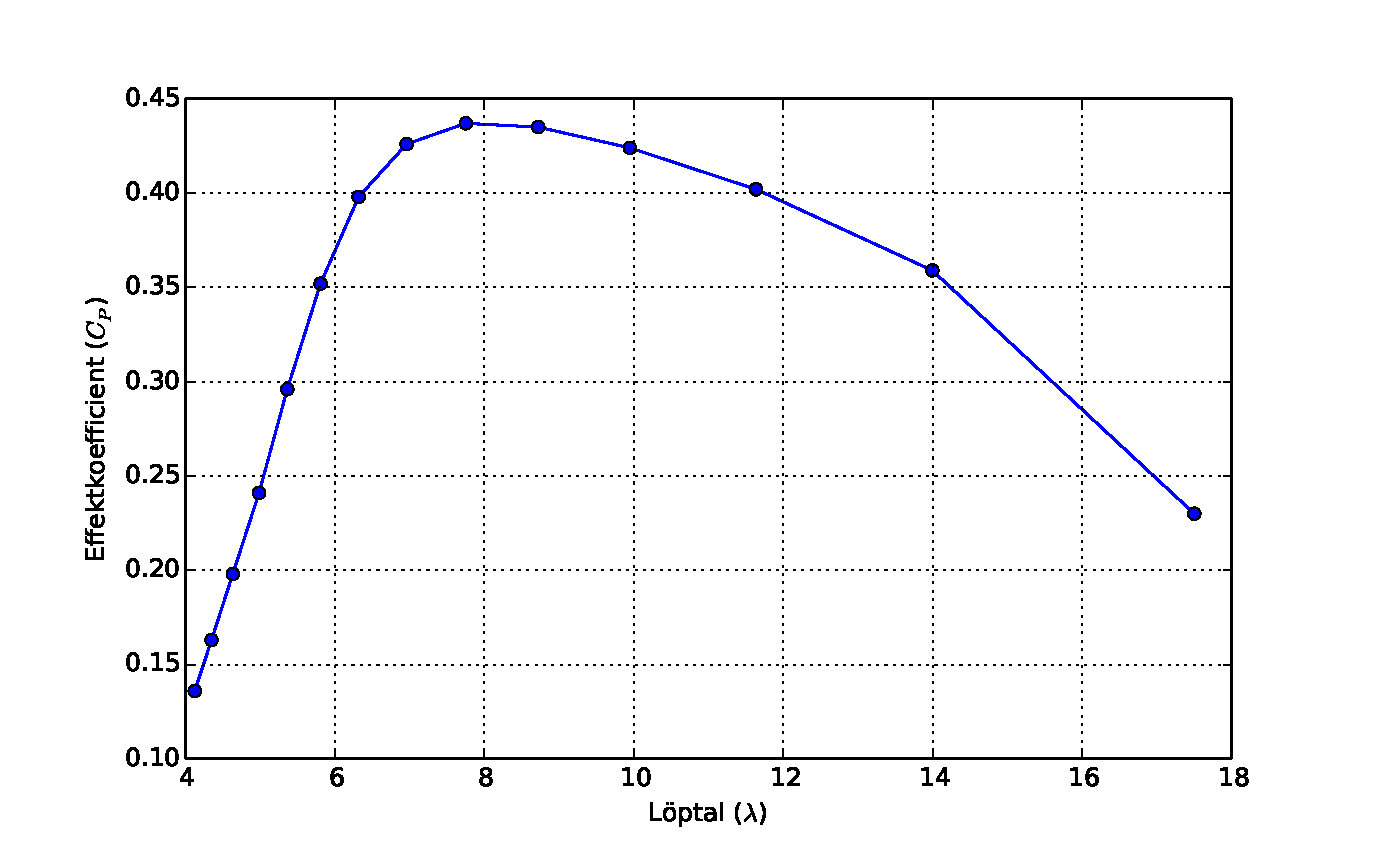
\includegraphics[width=11cm]{cpTSR.eps}
  \caption{$C_P$ mot $\lambda$ för Vestas V80 2 MW 80 m diameter. Fritt reproducerat från \citet{smallwindturbines}}
  \label{cpTSR}
\end{figure}

\pagebreak
\subsection{$C_l$- och $C_d$-kurvor}
\label{ClochCdkurvor}


$C_l$ och $C_d$ är på samma vis som tidigare en dimensionslös en storhet som beskriver lyftkraft och motståndskraft för en tvådimensionell vingprofil. Dessa definieras på följande sätt

\begin{equation}\label{c_l}
\begin{array}{cc}
C_l = \frac{l}{\frac{1}{2}\rho V_{tot}^2   c}, & C_d = \frac{d}{\frac{1}{2}\rho V_{tot}^2   c} \\ 
\end{array}
\end{equation}


Där $C_l$ och $C_d$ kommer visa sig beroende på vingprofilens utformning, $\alpha$ och $Re$. Typiska kurvor för deras starkaste beroende $\alpha$ visas i \fref{ClCd}. Här syns att vid ett speciellt $\alpha$ har $C_l$ nått sitt maximum och börjar minska. Detta kallas stall-vinkeln och kommer vidare benämnas $\alpha_{stall}$. 

\begin{figure}[!h]
  \centering
  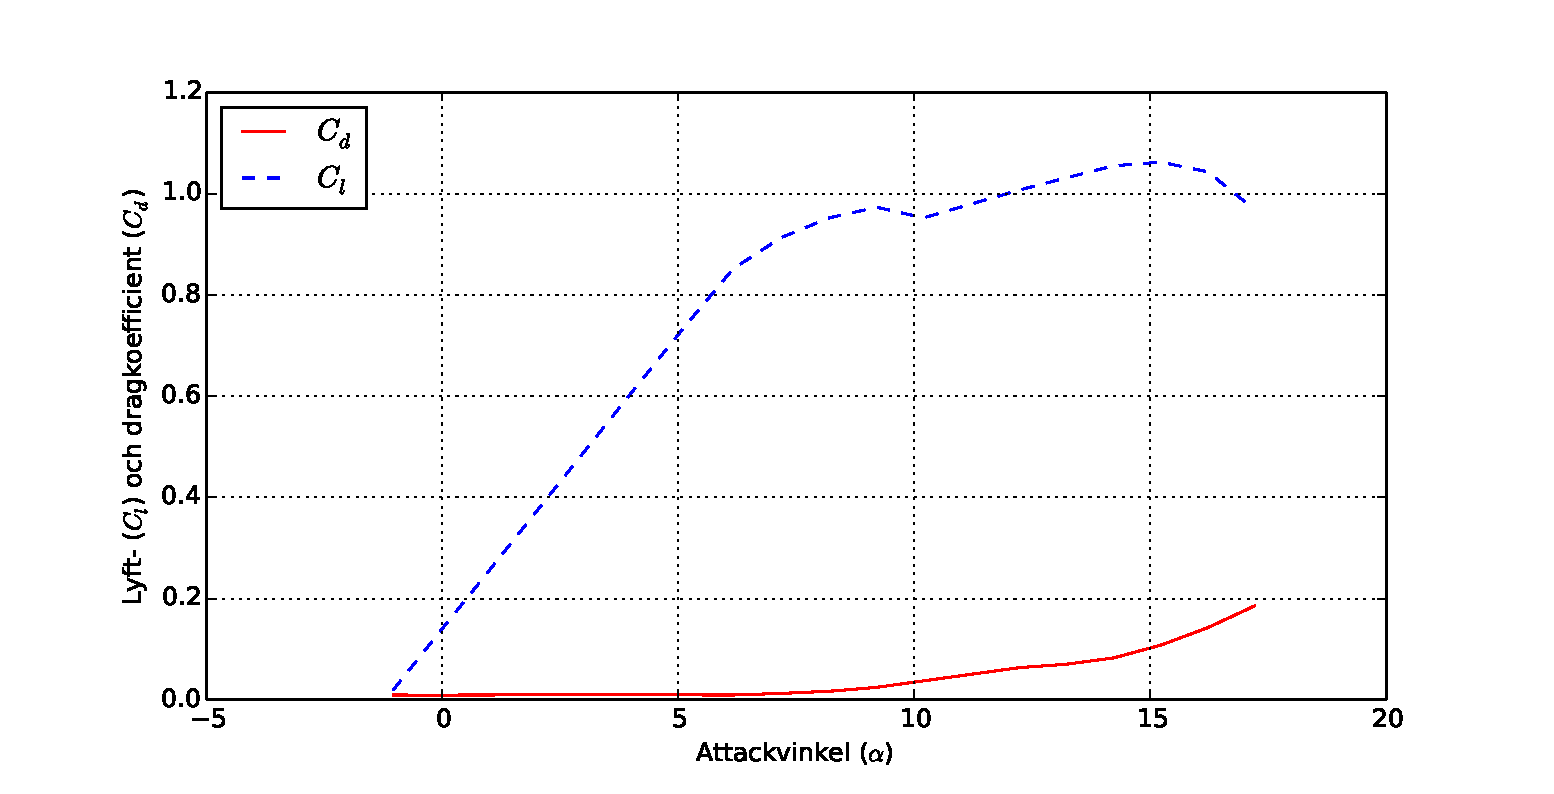
\includegraphics[width=12cm]{S809_Alfa_Cl_Cd}
  \caption{$C_l$ och $C_d$ för vingprofilen S809 vid $Re$ en miljon. Data från \citet{s809data}}
  \label{ClCd}
\end{figure}


Ekvationer som nu presenterats återfinns i mer utförlig form i \citet{smallwindturbines}. 



\subsection{Programvaror och erhållande av $C_l$ och $C_d$}
Lyft- och motståndskoefficient ($C_l$ och $C_d$) är de aerodynamiska variabler som är av högst intresse för att kunna göra en \textsc{Bem}-analys. Att ta fram dessa i vindtunnelexperiment är dock omöjligt i en optimeringsstudie som då hade inneburit att tusentals vingprofiler skulle byggas och testas i tunneln.

\textsc{cfd} (Computional Fluid Dynamics) är ett alternativ som ger resultat av hög kvalitet, men är ofta väldigt beräkningsintensivt. \cite{Xfoil} har utvecklat programvaran \textsc{Xfoil} som kan lösa det inviskösa och viskösa flödet kring en vingprofil. Detta genom en linjär vorticitetsmetod tillsammans med Karman-Tsien-kompesibilitetskorrektion löses det inviskösa flödet. Gränsskiktet och övergången till turbulent flöde löses simultant med det inviskösa potentialflödet med en global Newton–Raphson-metod.

Flertalet studier har undersökt \textsc{Xfoil}s giltighet och kunnat konstatera god överensstämmelse med verkligheten vid låga $\alpha$ \citep{CST, XfoilVerifikation}. \textsc{Xfoil} avviker enligt \citet{XfoilVerifikation} från experimentella resultat för $C_l$ nära och efter stallvinkeln passerats där $C_l$ då överskattas. Vid höga vinklar konstateras även att \textsc{Xfoil} underskattar $C_d$ och en korrektionsfaktor där \textsc{Xfoil} data ökas 10 \% används. Dock skulle inte denna korrektionsfaktor räcka till för att kompensera avvikelsen för $C_d$ som presenteras i \citet{CST}.


\subsection{Val av modell för att förutsäga ett vindkraftverks produktion}

Strömningen som uppstår kring ett vindkraftverks rotorblad är ofta av transient natur, turbulent, tredimensionellt samt med många separationer i flödet. Detta gör det till ett komplext problem som är väldigt tidsödande att lösa med \textsc{cfd} (Computional Fluid Dynamics). Ett alternativ till \textsc{cfd} är potentialteori, men då kan ingen hänsyn till fluidens viskositet tas. Därför har det blivit industristandard att idag använda ``blade element momentum''-teori (\textsc{Bem}). Detta är en tvådimensionell metod som i princip extrapoleras in i tre dimensioner tillsammans med semi-empiriska antaganden som kommer från jämförelser med \textsc{cfd}-studier. Detta leder till en metod som till väldigt låg beräkningskostnad kan ge tillräckligt goda förutsägelser på ett vindkraftverks elproduktion. \textsc{Bem}s största nackdel är att den inte tar hänsyn till vindens transienta natur utan förutsätter ett flöde i samma hastighet oberoende av tiden (stationärt tillstånd) samt en hastighet oberoende av position i rymden \citep{Qblade}. 

I \citet{bembraelleranus} visas att \textsc{Bem}s största felkälla är dess lyft- och motståndskoefficienter ($C_l$ och $C_d$). \textsc{Bem} kan alltså antas ge ett resultat nära verkligheten givet att lyft- och motståndskoefficienter är korrekta. Korrekta koefficienter kan ges med empiriska mätningar på vingprofiler i en vindtunnel. Tas dessa fram på annan väg bör resultatet för \textsc{Bem} beaktas med försiktighet.



\begin{comment}
\citet{UnsteadyWind} har visat att uppmätta resultat i vindtunnlar kan vara i underkant mot vad som sedan turbinen behöver klara ute i fält på grund av vindens stötvisa natur. Toppbelastningen visade sig vara högre än vad vindtunnelexperiment tillsammans med \textsc{Bem} förutsade vilket är en underliggande orsak till slitage i mekaniska delar som vindkraftverk dras med. 
\end{comment}






\subsection{Vingprofilsrepresentation}

    \begin{figure}[!h]
      \centering
      \includegraphics[width=0.7\textwidth]{connectTheDots}
      \caption{Vingprofilsrepresentation genom sammanbindning av diskreta punkter genom B-spline-interpolation}
      \label{connectTheDots}
    \end{figure}

Ett vindkraftverks rotorblad kan anses bestå av flera tvådimensionella vingprofiler. Det går att representera dessa vingprofiler på väldigt många olika sätt. Oftast görs detta med diskreta punkter som sammanbinds med någon interpolationsteknik (se \fref{connectTheDots}). Frihetsgrader benämner antalet parametrar som sedan kan förändras i optimeringsprocessen. En punkt i xy-planet är därmed förknippat med två frihetsgrader när punkten inte är låst i någon led. 

%% Undantaget är när en diskretiseringspunkt låses i x- eller y-ledd.

\citet{DrelaTrubbel} har visat att en allt för detaljerad representation av vingprofilen har många negativa effekter. Dels eftersom beräkningskostnaden växer med antalet parametrar som sedan optimeras över, men även eftersom optimeringen då kan börja ta hänsyn till små fysikaliska fenomen som borde vara obetydliga. I \citet{DrelaTrubbel}  utvecklades en vågformad yta på vingprofilen som uppstod för att kompensera för separationsbubblor. Dock är platsen för där separationsbubblorna uppstår beroende av $C_l$ och därför inte giltig för mer än just en angreppsvinkel på vingprofilen. \begin{comment}\hl{En vingprofil som inte är mjuk är ur tillverkningssynpunkt inte heller lämplig}.\end{comment} \citet{DrelaTrubbel} hade i sin studie 60 frihetsgrader på vingprofilsrepresentationen.

Av ovanstående anledningar används idag ett färre antal diskreta punkter. \citet{5MWkillen} använder som många andra \citep{LowRe,Grasso} bezierkurvor för denna interpolationen. Fördelarna är en mjuk representation av vingprofilen med få parametrar. \citet{5MWkillen} använder här 22 frihetsgrader men ner till 16 används \citep{Grasso}.

Liknande bezierkurvor är B-splines som även de ger en mjuk representation. Största skillnaden är att en förändring i en diskretiseringspunkt ger en mer lokal förändring på kurvan än vad motsvarande gör i en bezierkurva. \citet{Dansken} använder B-splines. 

\citet{Cencelli} har istället valt att definiera fem grundprofiler som sedan mixas efter olika proportioner. Detta inskränker således designrymden men har fördelen att frihetsgraderna minskar.

CST-metoden har i \citet{CST} använts vilket i princip är användandet av ett polynom för representationen. Koefficienterna i polynomet är således frihetsgraderna vilka kan hållas få till bekostnad på att alla vingprofiler inte kan representeras på detta sätt.

Andra författare har valt ytterligare förenklingar där t.ex. \citet{Victoria} valt att endast låta optimeringsalgoritmen välja ur en förutbestämd mängd vindprofiler (NACA 44XX).





\begin{comment}
\subsection{Programmeringsspråk}
Implementering av ett optimeringsproblem likt det studerade kan givetvis göras i vilket programmeringsspråk som helst. Trots det är det stor övervikt för \textsc{MatLab} \citep{CST, Cencelli, 5MWkillen}. \hl{Python används i en studie av de jag arbetat med, men då endast för att kalla på Fortran-rutiner} \citep{Victoria}. %\citet{5MWkillen} använder sig av NREL FAST vilket är en BEM-kod utvecklad i fortran.
\end{comment}

\subsection{``Blade element momentum''-teori (\textsc{Bem})}
\label{BEMlitt}

``Blade element momentum''-teori (\textsc{Bem}) är idag ett vanligt sätt att förutsäga ett vindkraftverks prestanda. Givet pitch-vinkel ($\theta$) och löptal ($\lambda$) kan effekt och tryckkraft uppskattas. För att kunna göra detta används två strömningsmekaniska teorier: Endimensionell rörelsemängdsteori och ``blade element''-teori som i kommande stycken beskrivs i korthet efter hur de formulerats i \citet{hansen}.

\subsubsection{Analys av rörelsemängd i en dimension}
\label{1dmomentumteori}

Denna teori beskriver en förenklad och ideal rotor som kan uppskattas till en cirkulär disk (d.v.s. oändligt antal rotorblad) utan tjocklek där strömningen är friktionsfri och inkompressibel. Det finns heller ingen rotationell hastighetskomponent i vaken bakom rotorn. Disken kommer att stanna upp vindhastigheten $V_{\infty}$ uppströms till $u$ i rotorplanet och till $u_1$ i vaken bakom rotorn. Trycket kommer att från atmosfärstrycket $p_0$ höjas till $p$ direkt innan rotorn för att sedan göra ett diskontinuerligt fall $\Delta p$. Hur tryck och vindhastighet varierar visas i \fref{tryckfall}.

\begin{figure}[!htb]
  \centering
  \includegraphics[width=0.9\textwidth]{tryckfall.pdf}
  \caption{Illustration visande strömlinjerna som passerar rotorn samt hur tryck och hastighet förändras över denna. Fritt reproducerat från \citet{hansen}.}
  \label{tryckfall}
\end{figure}

Tryckkraften $T$ ligger i strömningens riktning och är ett resultat av tryckfallet över rotorn.

\begin{equation}\label{thrust} T = \Delta p \pi R^2 \end{equation}

Bernoullis ekvation är nu giltig mellan platsen långt uppströms till precis innan rotorn,

\begin{equation}\label{fore}
p_0 + \frac{1}{2}\rho V_{\infty}^2 = p + \frac{1}{2}\rho u^2
\end{equation}

samt även mellan platsen precis bakom rotorn till långt nedströms,

\begin{equation}\label{efter}
p - \Delta p + \frac{1}{2}\rho u^2 = p_0 + \frac{1}{2} \rho u_1^2
\end{equation}

Kombineras dessa ekvationer erhålls

\begin{equation}\label{pdrop}
\Delta p = \frac{1}{2}\rho (V_{\infty}^2 - u_1^2)
\end{equation}

\begin{figure}[!htb]
  \centering
  \includegraphics[width=0.9\textwidth]{kontrollvolym.pdf}
  \caption{Kontrollvolym kring den ideala rotorn. Fritt reproducerat från \citet{hansen}.}
  \label{kontrollvolym}
\end{figure}

Ur en analys av en cirkulär kontrollvolym som visas i \fref{kontrollvolym} där stationärt flöde antas, atmosfärstrycket $p_o$ råder nedströms i vaken och att ingen radiell komponent av kraften uppstår kan följande visas

\begin{equation}\label{ekvkontrollvolym}
\rho u_1^2 A_1 + \rho V_{\infty}^2(A_{KV} - A_1) + \dot{m}_{sidan} V_{\infty} - \rho V_{\infty}^2 A_{KV} = -T
\end{equation}

Genom masskonservering kan $\dot{m}_{sidan}$ och totala massflödet $\dot{m}$ erhållas 

\begin{equations}
\begin{align}
        \label{msidan}\dot{m}_{sidan} &= \rho A_1 (V_{\infty} - u_1)\\
        \label{mprick}\dot{m} &= \rho u A = \rho u_1 A_1
\end{align}
\end{equations}

Genom att kombinera ekvationerna \ref{ekvkontrollvolym}, \ref{msidan} och \ref{mprick} fås

\begin{equation}\label{trusty}
T = \rho u A (V_{\infty} - u_1)
\end{equation}

Om $T$ nu ersätts med tryckfallet i ekvation \ref{thrust} fås

\begin{equation}\label{umedel}
u = \frac{1}{2} (V_{\infty} + u_1)
\end{equation}

Vilket visar att hastigheten i rotorplanet är ett medelvärde av friströmshastigheten och vakhastigheten.

\begin{figure}[!htb]
  \centering
  \includegraphics[width=0.9\textwidth]{kontrollvolym2.pdf}
  \caption{Ny kontrollvolym kring den ideala rotorn. Fritt reproducerat från \citet{hansen}. }
  \label{kontrollvolym2}
\end{figure}

Med kontrollvolymen i \fref{kontrollvolym2} och antagandet om ett friktionslöst flöde som inte har någon ändring i intern energi kan det nu visas att effekten i vindkraftverkets axel måste vara 

\begin{equation*}
P =  \underbrace{\rho u A}_{\dot{m}} \left(\frac{1}{2} V^2_{\infty} + \frac{p_0}{\rho} - \frac{1}{2} u^2_1 - \frac{p_0}{\rho}\right)
\end{equation*}

vilket ger

\begin{equation}\label{powwa}
P =  \frac{1}{2}\rho u A (V^2_{\infty} - u_1^2)
\end{equation}

Den axiella induktionsfaktorn $a$ kan nu introduceras som

\begin{equation}
a = \frac{V_{\infty} - u}{V_{\infty}}
\end{equation}

Genom att kombinera den med ekvation \ref{umedel} fås

\begin{equation}\label{adef}
a = \frac{V_{\infty} - u_1}{2 V_{\infty}}
\end{equation}

Detta kan nu introduceras i ekvation \ref{powwa} och \ref{trusty} och resulterar i

\begin{equation}\label{powermeda}
P = 2 \rho V^3_{\infty} a (1 - a)^2 A
\end{equation}

\begin{equation}
T = 2 \rho V^2_{\infty} a (1 - a) A
\end{equation}

$C_P$ är sedan tidigare definierat till 

\begin{equation}
C_P = \frac{P}{\frac{1}{2} \rho V^3_{\infty} A}
\end{equation}

Tillsammans med ekvation \ref{powermeda} och deriverat med avseende på $a$ samt satt lika med noll fås 

\begin{equation}
\frac{\operatorname{d}\!C_P}{\operatorname{d}\!a} = 4(1 - a)(1 - 3a) = 0
\end{equation}

Ur detta kan man se att $C_{P_{max}}$ uppstår när $a = 1/3$ varpå ett $C_P = 16/27 \approx 0.593$. Detta är känt under namnet Betz-gränsen vilket är ett teoretiskt maximum för hur mycket av vindens inneliggande energi som går att ta ut.

På samma sätt som $C_P$ introducerats definieras tryckkraftskoefficienten $C_T$

\begin{equation}
\label{CT}C_T = \frac{T}{\frac{1}{2} \rho V^2_{\infty} A}
\end{equation}

\begin{figure}[!htb]
  \centering
  \includegraphics[width=0.8\textwidth]{CT.pdf}
  \caption{Figur visande hur $C_T$ varierar med $a$. Fritt reproducerat från \citet{hansen}. }
  \label{CT}
\end{figure}

Antagandena som fram tills nu gjorts har med experimentella data visats endast giltiga för $a < 0.4$ vilket syns i \fref{CT}. Om rörelsemängsdteorin var giltig över 0.4 hade detta betytt att hastigheten i vaken var negativ vilket inte är fallet. Detta kommer senare att tas hänsyn till.

\begin{figure}[!htb]
  \centering
  \subfigure[Virveln ett flygplan inducerar. Foto: NASA public domain]{
    \includegraphics[height=4.2cm]{vortex}
    \label{vortex}
  }
  \subfigure[Virvlarna ett vindkraftverks rotorblad inducerar. Fritt reproducerat från \citet{hansen}]{
    \includegraphics[height=4.2cm]{virvlarfig.pdf}
    \label{virvlarfig}
  }
  \caption{Olika typer av virvlar.}
  \label{virvlar}
\end{figure}

$a$ som tidigare introducerades ska nu visa sig ha en fysikalisk betydelse som framöver är av stor vikt. I \fref{vortex} syns virveln som ett flygplans vinge inducerar. På samma sätt skapar ett vindkraftverks rotorblad virvlar som måste tas hänsyn till. I \fref{virvlarfig} illustreras dessa virvlar.

Systemet av virvlar inducerar en axiell hastighetskomponent i motsatt riktning som den inkommande vinden samt en tangentiell komponent i motsatt riktning till rotationen av rotorbladen. Den axiella hastigheten specificeras med den tidigare nämnda axiella induktionsfaktorn $a$ som $a V_{\infty}$. Den tangentiella hastigheten som uppstår i rotorns vak specificeras med den tangentiella induktionsfaktorn $a'$ som $2 a' \Omega r$.

$2 a' \Omega r$ kallas vidare $C_{\theta}$.

\begin{figure}[!htb]
  \centering
  \includegraphics[width=0.7\textwidth]{indushast.pdf}
  \caption{Hastighetskomponenterna som en vingprofil upplever. Fritt reproducerat från \citet{hansen}.}
  \label{indushast}
\end{figure}

Vingprofilerna i rotorbladet påverkas därför av hur dessa nya hastihetskomponenter beter sig. I \fref{indushast} syns dessa och följande samband gäller

\begin{equations}
\begin{align}
    V_a &= (1 - a)V_{\infty}\\
    V_{rot} &= (1 + a')\Omega r
\end{align}
\end{equations}

\subsubsection{``Blade element momentum''-metoden}

``Blade element momentum''-metoden kopplar samman den endimensionella rörelse-\\mängdsteorin med det som faktiskt händer lokalt längs bladet. Den kontrollvolymen som i endimensionella rörelsemängdsteorin introducerade delas nu upp i ett antal element med samma höjd $\operatorname{d}\!r$ där $r$ är den lokala radien och $R$ rotorns fulla radie. Detta ses i \fref{streamtubedr}. Dessa avgränsas av flödeslinjer vilket alltså betyder att inget flöde kan ske mellan dessa element vilket är ett antagande \textsc{Bem}-teorin vilar på.

\begin{figure}[!htb]
  \centering
  \includegraphics[width=0.7\textwidth]{streamtubedr.pdf}
  \caption{Kontrollvolym med formen som ett rör genom rotorplanet. Fritt reproducerat från \citet{hansen}.}
  \label{streamtubedr}
\end{figure}

Rörelsemängdsekvationen på integralform kan nu appliceras på ett element och ge tillskottet av tryckkraft i det elementet

\begin{equation}
\operatorname{d}\!T = (V_{\infty} - u_1)\operatorname{d}\!\dot{m} = 2 \pi r \rho u (V_{\infty} - u_1)\operatorname{d}\!r
\end{equation}

Vridmomentet $\operatorname{d}\!Q$ kan på samma sätt tas fram om rotationens hastighet i friströmmen sätts till noll och den i vaken sätts till $C_{\theta}$

\begin{equation}
\operatorname{d}\!Q = r C_{\theta} \operatorname{d}\!m = 2 \pi r^2 \rho u C_{\theta} \operatorname{d}\!r
\end{equation}

Genom att nu föra in det som tagits fram gällande $a$ i ekvation \ref{adef} samt $C_{\theta} = 2 a' \Omega r$ kan tryckkraft och vridmoment skrivas om till

\begin{equations}
\begin{align}
\label{firstdT}\operatorname{d}\!T &= 4 \pi r \rho V_{\infty}^2 a (1 - a) \operatorname{d}\!r \\
\label{firstdQ}\operatorname{d}\!Q &= 4 \pi r^3 \rho V_{\infty} \Omega (1 - a) a' \operatorname{d}\!r 
\end{align}
\end{equations}

\begin{figure}[!htb]
  \centering
  \includegraphics[width=0.9\textwidth]{vrotva.pdf}
  \caption{Hastighetskomponenterna en vingprofil i rotorplanet upplever. Fritt reproducerat från \citet{hansen}.}
  \label{vrotva}
\end{figure}

Om nu $V_{rot}$ och $V_a$ placeras ut som i \fref{vrotva} kan ses att vingprofilen i själva verket utsätts för hastigheten $V_{tot}$. \emph{Pitch} i varje lokal vingprofil längs rotorbladet är en kombination av bladets \emph{pitch} ($\theta_p$) och \emph{twist} ($\beta$) som $\theta = \theta_p + \beta$. $\phi$ är den totala vinkeln mellan rotorplanet och hastigheten $V_{tot}$.

Vingprofilens lokala angreppsvinkel ($\alpha$) blir alltså

\begin{equation*}
\alpha = \phi - \theta
\end{equation*}

\fref{vrotva} ger även att 

\begin{equation*}
\phi = \arctan \frac{(1 - a)V_{\infty}}{(1 + a')\Omega r}
\end{equation*}

Lyft- och motståndskraften har tidigare visas implicit i \ref{c_l}. Lyftkraften ligger vinkelrätt mot den inkommande vindhastigheten $V_{tot}$ och motståndskraften i samma riktning. Därför gäller

\begin{equations}
\begin{align}
    l = \frac{1}{2} \rho V_{tot}^2 c C_l \\
    d = \frac{1}{2} \rho V_{tot}^2 c C_d
\end{align}
\end{equations}

Där små bokstäver för lyft- och motståndskraft används för att påpeka att det är tvådimensionella krafter.

\begin{figure}[!htb]
  \centering
  \includegraphics[width=0.8\textwidth]{liftdragproj.pdf}
  \caption{Krafter upplevda av en vingprofil i rotorplanet. Fritt reproducerat från \citet{hansen}.}
  \label{liftdragproj}
\end{figure}

Eftersom endast normal- och tangentialkraften i rotorplanet är av intresse projiceras krafterna till $F_n$ och $F_t$ vilket syns i \fref{liftdragproj} enligt

\begin{equations}
\begin{align}
    F_n &= l \cos \phi + d \sin \phi  \\
    F_t &= l \sin \phi - d \cos \phi
\end{align}
\end{equations}

Dessa kan nu göras dimensionslösa genom att delas på $\frac{1}{2} \rho V_{tot}^2 c$ och blir då

\begin{equations}
\begin{align}
\label{Cn} C_n &= C_l \cos \phi + C_d \sin \phi  \\
\label{Ct} C_t &= C_l \sin \phi - C_d \cos \phi
\end{align}
\end{equations}

där 

\begin{equations}
\begin{align}
\label{Cn2} C_n &= \frac{F_n}{\frac{1}{2}\rho V_{tot}^2 c}\\
\label{Ct2} C_t &= \frac{F_t}{\frac{1}{2}\rho V_{tot}^2 c}
\end{align}
\end{equations}

Ur geometrin i \fref{vrotva} kan även ses att 

\begin{equations}
\begin{align}
\label{vtotsin} V_{tot} \sin \phi &= V_{\infty} (1 - a) \\
\label{vtotcos}V_{tot} \cos \phi &= \Omega r (1 + a')
\end{align}
\end{equations}

Lokal \emph{solidity} $\sigma$ införs som andelen yta som täcks med blad i en radiell position

\begin{equation}
\label{solidity}\sigma (r) = \frac{c(r)B}{2 \pi r}
\end{equation}

Notera att detta är lokalt vid varje position på rotorbladet och därför en funktion av radien. $B$ är antalet blad på vindkraftverket, $c(r)$ den lokala kordan och $r$ den radiella positionen.

Krafterna $F_n$ och $F_t$ multipliceras eftersom de är tvådimensionella med sitt radiella element $\operatorname{d}\!r$ och ger tillskottet av \emph{trust} $\operatorname{d}\!T$ och vridmoment $\operatorname{d}\!Q$

\begin{equations}
\begin{align}
    \operatorname{d}\!T &= B F_n \operatorname{d}\!r \\
\label{dQen}\operatorname{d}\!Q &= r B F_t \operatorname{d}\!r
\end{align}
\end{equations}

Använder ekvation \ref{Cn2} för att ersätta $F_n$ och ekvation \ref{vtotsin} för $V_{tot}$ fås istället

\begin{equation}
\label{dTkrongling}\operatorname{d}\!T = \frac{1}{2}\rho B \frac{V_{\infty}^2(1 - a)^2}{\sin^2 \phi} c C_n \operatorname{d}\!r
\end{equation}

Används på liknande sätt ekvation \ref{Ct2} för att ersätta $F_t$ och ekvation \ref{vtotsin} och \ref{vtotcos} blir nu istället \ref{dQen}

\begin{equation}
\label{dQkrongling}\operatorname{d}\!Q = \frac{1}{2}\rho B \frac{V_{\infty} (1 - a) \Omega r (1 + a')}{\sin \phi \cos \phi} c C_t r \operatorname{d}\!r
\end{equation}

Likställs $dT$ för \ref{firstdT} och \ref{dTkrongling} samt appliceras $\sigma$ (\ref{solidity}) kan ett utryck för $a$ nu härledas

\begin{equation}
\label{finala} a = \frac{1}{\frac{4 \sin^2 \phi}{\sigma C_n} + 1}
\end{equation}

Om \ref{firstdQ} och \ref{dQkrongling} likställs fås på samma sätt 

\begin{equation}
\label{finala} a' = \frac{1}{\frac{4 \sin \phi \cos \phi}{\sigma C_t} - 1}
\end{equation}

\subsubsection{Prantl topp-förluster}

Tidigare i \ref{1dmomentumteori} har antaganden gjorts att vindkraftverkets rotor bestått av ett oändligt antal rotorblad. När ett begränsat antal rotorblad som t.ex. 3 st används påverkar detta virvlarna som uppstår i vaken. För att kompensera för detta används ofta Prandtls korrektionsfaktor $F$. För en fullständig härledning hänvisas läsaren till \citet{glauert}.

\begin{equation}
\label{F} f = \frac{B}{2} \frac{R-r}{r \sin \phi}
\end{equation}

Sätts in i

\begin{equation}
\label{F} F = \frac{2}{\pi} \arccos (e^{-f}) 
\end{equation}

Om ekvation \ref{firstdT} och \ref{firstdQ} multipliceras med $F$ och $a$ och $a'$ löses ut fås istället

\begin{equations}
\begin{align}
   \label{aFkorrad} a &= \frac{1}{\frac{4 F \sin^2 \phi}{\sigma C_n} + 1} \\
   \label{aprimkorrad} a' &= \frac{1}{\frac{4 F \sin \phi \cos \phi}{\sigma C_t} - 1}
\end{align}
\end{equations}

\subsubsection{Glauert-korrektion}

I \fref{CT} visades att för $a > 0.4$ behövs en empirisk korrektion göras för $C_T$. Detta görs enligt förfarandet föreslagit i \citet{buhl} eftersom annars en numerisk instabilitet kan uppstå \citep{adyntheory}.

När $C_T > 0.96F$ vilket är samma som $a > 0.4$ gäller därför 

\begin{equation}
\label{aKorr} a = \frac{18F-20-3\sqrt{C_T(50-36F) + 12F(3F-4)}}{36F-50}
\end{equation}

$C_T$ tas nu istället fram genom att sätta samman dess definition \ref{CT} för ett radiellt element 

\begin{equation}
C_T = \frac{\operatorname{d}\!T}{ \rho V^2_{\infty} \pi \operatorname{d}\!r}
\end{equation}

med \ref{dTkrongling} vilket ger

\begin{equation}
\label{CTNY}C_T = \frac{(1 - a)^2\sigma C_n}{\sin^2 \phi}
\end{equation}


\pagebreak
\subsubsection{Implementering av \textsc{Bem}-algoritmen}

Alla ekvationer som behövs har nu presenterats och $a$ och $a'$ kan nu iterativt tas fram för varje radiellt element på rotorn. Detta görs förslagsvis enligt följande steg:

\begin{enumerate}
  \item Initialt sätts $a = 0$ och $a' = 0$
  \item Vinkeln $\phi = \arctan \frac{(1 - a)V_{\infty}}{(1 + a')\Omega r}$ beräknas så att $\alpha = \phi - \theta$ kan tas fram.
  \item $C_l$ och $C_d$ interpoleras fram från datan som i denna studie kommer från \textsc{Xfoil}. 
  \item $C_n$ och $C_t$ beräknas enligt ekvationerna \ref{Cn} och \ref{Ct}.
  \item Räkna ut Prantl topp-förlust-faktorn $F$ genom ekvation \ref{F} samt $C_T$ med ekvation \ref{CTNY}
  \item Beroende på värde på $C_T$ beräkna $a$ med ekvation \ref{aKorr} eller \ref{aFkorrad}.
  \item Räkna ut $a'$ med ekvation \ref{aprimkorrad}
  \item Jämför värdet på $a$ med det tidigare. Skiljer de sig mindre åt än tolleransnivån har konvergens nåtts. Om inte, gå tillbaka till steg 2.
  \end{enumerate}
  
När $a$ och $a'$ erhållits för alla radiella element längs rotorn kan nu även vridmomentet för alla radiella element beräknas med exempelvis ekvation \ref{dQkrongling}.

Genom att sedan integrera dessa tillskott $\operatorname{d}\!Q$ till vridmomentet, och med antagandet att allt före $r_{hub}$ endast genererar motståndskraft - fås det totala vridmomentet i rotorn. 

\begin{equation}
Q = \int_{r_{hub}}^R \operatorname{d}\!Q
\end{equation}

Detta används tillsammans med vinkelhastigheten ($\Omega$) för att få fram rotorns effekt

\begin{equation}
P = Q \Omega
\end{equation}

För mer utförlig beskrivning av ekvationer som här presenterats hänvisas läsaren till \citet{wehb}.
  


\subsection{Optimeringslära}

Studiens mål och senare metodologi  baseras att ett optimeringsproblem där så mycket effekt som möjligt ska tas ut ur vinden. Därför presenteras här optimeringsterminologi och optimeringsalgoritmer som senare används.

\begin{figure}[!htb]
  \centering
  \includegraphics[width=0.9\textwidth]{designmalrymd}
  \caption{Illustration visande hur designrymden utvärderas av målfunktionen för att ge en målrymd.}
  \label{designmalrymd}
\end{figure}

Ett optimeringsproblem definieras av sina designvariabler, designrymd, dess målfunktion och målrymd (se \fref{designmalrymd}). Designvariablerna utgör de variabler som kan varieras för för att få olika resultat. Givet $N$ antal designvariabler $\left\{f_1, f_2, \dots, f_N\right\}$ (i \fref{designmalrymd} är $N=2$) definieras designrymden varpå målfunktionen utvärderar dessa för att returnera en målrymd. I denna studien är målrymden endast ett reellt tal eftersom optimeringen av vindkraftverkets rotorblad endast görs med avseende på dess genomsnittliga effekt $\overline{P}$. Eftersom målfunktionen maximeras kallas ibland även målfunktionen för \emph{fitness-funktion}.

\subsubsection{Andra författares val av målfunktion}

Valet av ett optimeringsproblems målfunktion är av yttersta vikt för vilket resultat som kommer fås. \citet{Dansken, LowRe, Grasso} optimerar endast en vingprofils lyft- och motståndskoefficienter ($C_l$ och $C_d$) över rimliga angreppsvinklar. \citet{Cencelli} gör optimeringen på vindkraftverkets effektkoefficient ($C_P$) vid ett par olika vindhastigheter. 

Andra författare tar ett större grepp och väljer att maximera ett vindkraftverks årliga produktion. \citet{Victoria} låter ett vindhastighetshistogram vara styrande. Detta är ett intressant förhållningssätt eftersom vindkraftverkets riktiga produktion för en specifik plats då nås. Effektkurvan matchas då med vindhastighetshistogrammet som beskriver andelen av tid som en viss vindhastighet förekommer varpå genomsnittseffekten $\overline{P}$ kan tas fram.

\subsubsection{Optimeringsalgoritmer}
Lämpliga optimeringsmetoder som studerats har antingen använt sig av gradient för optimeringen eller inte. I \citet{Victoria} används gradientmetoden SQP (sequential quadratic programming). Fördelen är att konvergens snabbare kan uppnås med en gradient som visar i vilken riktning optimeringen bör fortskrida, men har den stora nackdelen att lokala max/min ofta står för konvergensen. 

Därför är genetiska algoritmer väldigt återkommande i den studerade litteraturen då de är en metod som når globala max/min \citep{Benini, 5MWkillen, LowRe, CST, Dansken}. Flera varianter på genetiska algoritmer finns. ECGA är en variant på genetisk algoritm som utlovar snabbare konvergens med mindre populationsstorlekar \citep{Xiong}. \citet{Grasso} utlovar samma sak med det som kallas microGA.

``Particle swarm''-metoden är även den en gradientlös metod som imiterar ett flockdjurs tendens att efterlikna andra individers framgångsrika beteende. I \citet{Cencelli} används metoden framgångsrikt.  



\subsubsection{Genetiska algoritmer}

En genetisk algoritm är en optimering som hämtar terminologi och inspiration från evolutionen som sker i naturen. Principen är att individer med goda egenskaper kommer premieras i evolutionen genom att deras arvsmassa förs vidare i större utsträckning än mindre lyckade individer.

Följande begrepp är centrala och dess betydelse listas här:

\begin{description}
  \item[Individ] En möjlig lösning på optimeringsproblemet. I denna studie kommer varje individ vara ett vindkraftverk.
  \item[Population] En grupp av individer.
  \item[Arvsmassa] En individs bakomliggande genetiska uppsättning som ger upphov till individens egenskaper. I detta fallet är det vindkraftverkets vingprofiler, korda-distribution och \emph{twist}-distribution längs rotorbladet. Detta representeras av en sträng siffror eller bokstäver $G = \left\{ g_1, g_2, \dots, g_n\right\}$.
  \item[\emph{Fitness}-funktion] Målfunktionen som utvärderar individerna. 
\end{description}

En initial population individer inleder den genetiska algoritmen. Hur bra en individ är, avgörs av den så kallade \emph{fitness}-funktionen som i denna studien utgörs av \textsc{Bem}-algoritmen. 

När alla individer har tilldelats ett \emph{fitness}-värde kan individerna ordnade efter \emph{fitness} tilldelas en partner som deras arvsmassa blandas med enligt en förutbestämd sannolikhet. Vid korsningen av arvsmassa sker även vissa mutationer med en bestämd sannolikhet. Efter detta sker \emph{fitness}-utvärderingen på nytt och proceduren upprepas tills ett förutbestämt antal generationer passerat eller att ett \emph{fitness}-mål uppnås.


\section{Relevans för studien}
I litteraturstudien har det framkommit att optimering av ett vindkraftverk ofta görs med målfunktioner som inte representerar produktionen för ett vindkraftverk på ett specifikt vindförhållande. Det är därför rimligt att i optimeringen fortsätta ta hänsyn till vindhastighetsfördelningen vilket utifrån litteraturstudien  endast \citet{Victoria} gör. \citet{Victoria} har en väldigt begränsad designrymd där endast vingprofiler i NACA 44XX-serien används. Detta bjuder in till att ta vid där de slutade och utöka med en större designrymd med fler vingprofiler.

%% Hör inte hemma. Kan jag komma på en annan vinkel för Fritt reproducerat frånp?
\begin{comment}Det stora antalet sätt att representera vingprofiler är en produkt av att tidigare författare försökt hitta representationer med så få parametrar som möjligt utan för den delen inskränka designrymden. Detta 

%% ----

\rework{Python är ett kraftfullt, enkelt programmeringsspråk med högt pedagogiskt värde då koden är lättläst även för den som inte kan Python. Att använda Python som programmeringsspråk är därmed ett medvetet val där det till skillnad från t.ex. \textsc{MatLab} även är helt öppet. En kommersiell licens för \textsc{MatLab} kostar idag 17 500 \citep{MATLAB} vilket begränsar tillgången för de utan medel. Mitt program kommer därför vara helt oförknippat med några kostnader.}

\end{comment}

\section{Avgränsningar}
\textsc{Xfoil} har visat sig vara ett välanvänt alternativ för att ta fram en vingprofils aerodynamiska egenskaper. Eftersom resultaten visats vara goda kommer inga utförliga försök till att verifiera \textsc{Xfoil}s giltighet att göras. Vidare kommer inga andra programvaror att beaktats eftersom litteraturstudien även visat att t.ex. \textsc{cfd} kommer till för stor beräkningskostnad.

I denna studie beaktas uteslutande vindhastighet som oberoende av rumskoordinater och vid stationärt tillstånd då detta är förutsättningar för \textsc{Bem}. 

Luft betraktas i studien som en inkompressibel fluid. Detta trots att vindhastigheter vid vingbladens topp på vindkraftverk av megawatt-klass kan komma så långt som mach 0.25-0.3 \citep{XfoilVerifikation}.

Strukturella aspekter som belastningen i rotorbladets struktur tas med i ett par studier och kan ge betydande påverkan på resultatet \citep{5MWkillen, Victoria}. Detta kommer här anses ligga utanför studiens omfattning för att istället tas hänsyn till med enklare restriktioner.

Mer avancerade genetiska algoritmer har framkommit i litteraturstudien, men en mer djupgående analys av deras skillnader anses ligga utanför denna rapportens ambition.



